% generated by Plantuml 1.2024.4       
\definecolor{plantucolor0000}{RGB}{241,241,241}
\definecolor{plantucolor0001}{RGB}{24,24,24}
\definecolor{plantucolor0002}{RGB}{173,209,178}
\definecolor{plantucolor0003}{RGB}{0,0,0}
\definecolor{plantucolor0004}{RGB}{200,41,48}
\definecolor{plantucolor0005}{RGB}{3,128,72}
\definecolor{plantucolor0006}{RGB}{132,190,132}
\scalebox{0.7442}{
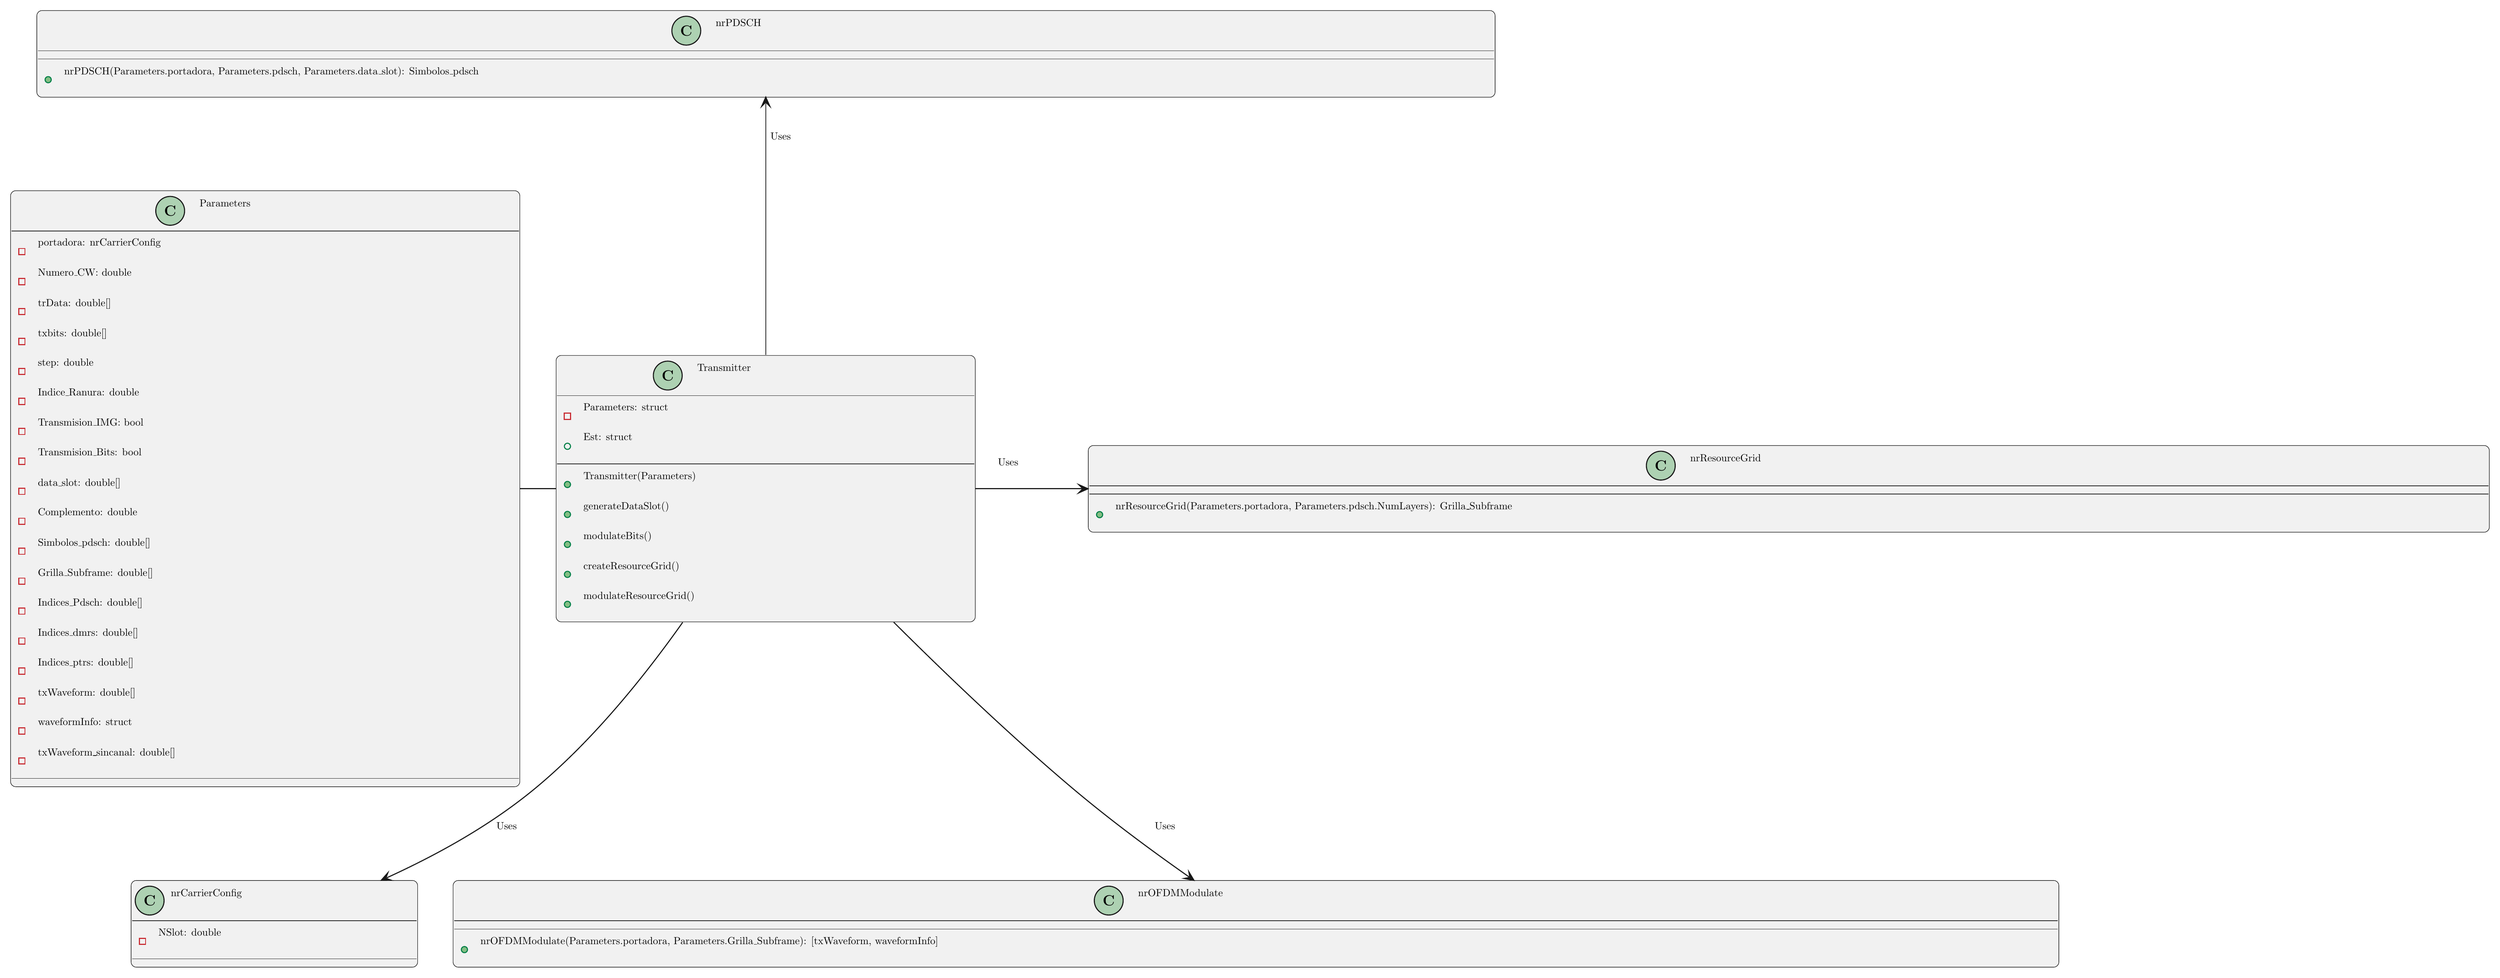
\begin{tikzpicture}[yscale=-1
,pstyle0/.style={color=plantucolor0001,fill=plantucolor0000,line width=0.5pt}
,pstyle1/.style={color=plantucolor0001,fill=plantucolor0002,line width=1.0pt}
,pstyle2/.style={color=plantucolor0001,line width=0.5pt}
,pstyle3/.style={color=plantucolor0004,line width=1.0pt}
,pstyle5/.style={color=plantucolor0005,fill=plantucolor0006,line width=1.0pt}
,pstyle6/.style={color=plantucolor0001,line width=1.0pt}
,pstyle7/.style={color=plantucolor0001,fill=plantucolor0001,line width=1.0pt}
]
\draw[pstyle0] (536.5pt,347pt) arc (180:270:5pt) -- (541.5pt,342pt) -- (938.325pt,342pt) arc (270:360:5pt) -- (943.325pt,347pt) -- (943.325pt,595.8125pt) arc (0:90:5pt) -- (938.325pt,600.8125pt) -- (541.5pt,600.8125pt) arc (90:180:5pt) -- (536.5pt,595.8125pt) -- cycle;
\draw[pstyle1] (644.8704pt,361.5508pt) ellipse (14pt and 14pt);
\node at (644.8704pt,361.5508pt)[]{\textbf{\Large C}};
\node at (669.8704pt,347pt)[below right,color=black]{Transmitter};
\draw[pstyle2] (537.5pt,381.1016pt) -- (942.325pt,381.1016pt);
\draw[pstyle3] (544.5pt,398.1523pt) rectangle (550.5pt,404.1523pt);
\node at (559.5pt,385.1016pt)[below right,color=black]{Parameters: struct};
\draw[color=plantucolor0005,line width=1.0pt] (547.5pt,430.2539pt) ellipse (3pt and 3pt);
\node at (559.5pt,414.2031pt)[below right,color=black]{Est: struct};
\draw[pstyle2] (537.5pt,447.3047pt) -- (942.325pt,447.3047pt);
\draw[pstyle5] (547.5pt,467.3555pt) ellipse (3pt and 3pt);
\node at (559.5pt,451.3047pt)[below right,color=black]{Transmitter(Parameters)};
\draw[pstyle5] (547.5pt,496.457pt) ellipse (3pt and 3pt);
\node at (559.5pt,480.4063pt)[below right,color=black]{generateDataSlot()};
\draw[pstyle5] (547.5pt,525.5586pt) ellipse (3pt and 3pt);
\node at (559.5pt,509.5078pt)[below right,color=black]{modulateBits()};
\draw[pstyle5] (547.5pt,554.6602pt) ellipse (3pt and 3pt);
\node at (559.5pt,538.6094pt)[below right,color=black]{createResourceGrid()};
\draw[pstyle5] (547.5pt,583.7617pt) ellipse (3pt and 3pt);
\node at (559.5pt,567.7109pt)[below right,color=black]{modulateResourceGrid()};
\draw[pstyle0] (7pt,187pt) arc (180:270:5pt) -- (12pt,182pt) -- (496.2873pt,182pt) arc (270:360:5pt) -- (501.2873pt,187pt) -- (501.2873pt,755.9297pt) arc (0:90:5pt) -- (496.2873pt,760.9297pt) -- (12pt,760.9297pt) arc (90:180:5pt) -- (7pt,755.9297pt) -- cycle;
\draw[pstyle1] (161.9247pt,201.5508pt) ellipse (14pt and 14pt);
\node at (161.9247pt,201.5508pt)[]{\textbf{\Large C}};
\node at (186.9247pt,187pt)[below right,color=black]{Parameters};
\draw[pstyle2] (8pt,221.1016pt) -- (500.2873pt,221.1016pt);
\draw[pstyle3] (15pt,238.1523pt) rectangle (21pt,244.1523pt);
\node at (30pt,225.1016pt)[below right,color=black]{portadora: nrCarrierConfig};
\draw[pstyle3] (15pt,267.2539pt) rectangle (21pt,273.2539pt);
\node at (30pt,254.2031pt)[below right,color=black]{Numero\_CW: double};
\draw[pstyle3] (15pt,296.3555pt) rectangle (21pt,302.3555pt);
\node at (30pt,283.3047pt)[below right,color=black]{trData: double[]};
\draw[pstyle3] (15pt,325.457pt) rectangle (21pt,331.457pt);
\node at (30pt,312.4063pt)[below right,color=black]{txbits: double[]};
\draw[pstyle3] (15pt,354.5586pt) rectangle (21pt,360.5586pt);
\node at (30pt,341.5078pt)[below right,color=black]{step: double};
\draw[pstyle3] (15pt,383.6602pt) rectangle (21pt,389.6602pt);
\node at (30pt,370.6094pt)[below right,color=black]{Indice\_Ranura: double};
\draw[pstyle3] (15pt,412.7617pt) rectangle (21pt,418.7617pt);
\node at (30pt,399.7109pt)[below right,color=black]{Transmision\_IMG: bool};
\draw[pstyle3] (15pt,441.8633pt) rectangle (21pt,447.8633pt);
\node at (30pt,428.8125pt)[below right,color=black]{Transmision\_Bits: bool};
\draw[pstyle3] (15pt,470.9648pt) rectangle (21pt,476.9648pt);
\node at (30pt,457.9141pt)[below right,color=black]{data\_slot: double[]};
\draw[pstyle3] (15pt,500.0664pt) rectangle (21pt,506.0664pt);
\node at (30pt,487.0156pt)[below right,color=black]{Complemento: double};
\draw[pstyle3] (15pt,529.168pt) rectangle (21pt,535.168pt);
\node at (30pt,516.1172pt)[below right,color=black]{Simbolos\_pdsch: double[]};
\draw[pstyle3] (15pt,558.2695pt) rectangle (21pt,564.2695pt);
\node at (30pt,545.2188pt)[below right,color=black]{Grilla\_Subframe: double[]};
\draw[pstyle3] (15pt,587.3711pt) rectangle (21pt,593.3711pt);
\node at (30pt,574.3203pt)[below right,color=black]{Indices\_Pdsch: double[]};
\draw[pstyle3] (15pt,616.4727pt) rectangle (21pt,622.4727pt);
\node at (30pt,603.4219pt)[below right,color=black]{Indices\_dmrs: double[]};
\draw[pstyle3] (15pt,645.5742pt) rectangle (21pt,651.5742pt);
\node at (30pt,632.5234pt)[below right,color=black]{Indices\_ptrs: double[]};
\draw[pstyle3] (15pt,674.6758pt) rectangle (21pt,680.6758pt);
\node at (30pt,661.625pt)[below right,color=black]{txWaveform: double[]};
\draw[pstyle3] (15pt,703.7773pt) rectangle (21pt,709.7773pt);
\node at (30pt,690.7266pt)[below right,color=black]{waveformInfo: struct};
\draw[pstyle3] (15pt,732.8789pt) rectangle (21pt,738.8789pt);
\node at (30pt,719.8281pt)[below right,color=black]{txWaveform\_sincanal: double[]};
\draw[pstyle2] (8pt,752.9297pt) -- (500.2873pt,752.9297pt);
\draw[pstyle0] (124pt,857pt) arc (180:270:5pt) -- (129pt,852pt) -- (397.0941pt,852pt) arc (270:360:5pt) -- (402.0941pt,857pt) -- (402.0941pt,931.2031pt) arc (0:90:5pt) -- (397.0941pt,936.2031pt) -- (129pt,936.2031pt) arc (90:180:5pt) -- (124pt,931.2031pt) -- cycle;
\draw[pstyle1] (142pt,871.5508pt) ellipse (14pt and 14pt);
\node at (142pt,871.5508pt)[]{\textbf{\Large C}};
\node at (159pt,857pt)[below right,color=black]{nrCarrierConfig};
\draw[pstyle2] (125pt,891.1016pt) -- (401.0941pt,891.1016pt);
\draw[pstyle3] (132pt,908.1523pt) rectangle (138pt,914.1523pt);
\node at (147pt,895.1016pt)[below right,color=black]{NSlot: double};
\draw[pstyle2] (125pt,928.2031pt) -- (401.0941pt,928.2031pt);
\draw[pstyle0] (436.5pt,857pt) arc (180:270:5pt) -- (441.5pt,852pt) -- (1990.0419pt,852pt) arc (270:360:5pt) -- (1995.0419pt,857pt) -- (1995.0419pt,931.2031pt) arc (0:90:5pt) -- (1990.0419pt,936.2031pt) -- (441.5pt,936.2031pt) arc (90:180:5pt) -- (436.5pt,931.2031pt) -- cycle;
\draw[pstyle1] (1072.8594pt,871.5508pt) ellipse (14pt and 14pt);
\node at (1072.8594pt,871.5508pt)[]{\textbf{\Large C}};
\node at (1097.8594pt,857pt)[below right,color=black]{nrOFDMModulate};
\draw[pstyle2] (437.5pt,891.1016pt) -- (1994.0419pt,891.1016pt);
\draw[pstyle2] (437.5pt,899.1016pt) -- (1994.0419pt,899.1016pt);
\draw[pstyle5] (447.5pt,919.1523pt) ellipse (3pt and 3pt);
\node at (459.5pt,903.1016pt)[below right,color=black]{nrOFDMModulate(Parameters.portadora, Parameters.Grilla\_Subframe): [txWaveform, waveformInfo]};
\draw[pstyle0] (32.5pt,12pt) arc (180:270:5pt) -- (37.5pt,7pt) -- (1442.8599pt,7pt) arc (270:360:5pt) -- (1447.8599pt,12pt) -- (1447.8599pt,86.2031pt) arc (0:90:5pt) -- (1442.8599pt,91.2031pt) -- (37.5pt,91.2031pt) arc (90:180:5pt) -- (32.5pt,86.2031pt) -- cycle;
\draw[pstyle1] (662.8596pt,26.5508pt) ellipse (14pt and 14pt);
\node at (662.8596pt,26.5508pt)[]{\textbf{\Large C}};
\node at (687.8596pt,12pt)[below right,color=black]{nrPDSCH};
\draw[pstyle2] (33.5pt,46.1016pt) -- (1446.8599pt,46.1016pt);
\draw[pstyle2] (33.5pt,54.1016pt) -- (1446.8599pt,54.1016pt);
\draw[pstyle5] (43.5pt,74.1523pt) ellipse (3pt and 3pt);
\node at (55.5pt,58.1016pt)[below right,color=black]{nrPDSCH(Parameters.portadora, Parameters.pdsch, Parameters.data\_slot): Simbolos\_pdsch};
\draw[pstyle0] (1053pt,434.5pt) arc (180:270:5pt) -- (1058pt,429.5pt) -- (2407.8496pt,429.5pt) arc (270:360:5pt) -- (2412.8496pt,434.5pt) -- (2412.8496pt,508.7031pt) arc (0:90:5pt) -- (2407.8496pt,513.7031pt) -- (1058pt,513.7031pt) arc (90:180:5pt) -- (1053pt,508.7031pt) -- cycle;
\draw[pstyle1] (1608.6864pt,449.0508pt) ellipse (14pt and 14pt);
\node at (1608.6864pt,449.0508pt)[]{\textbf{\Large C}};
\node at (1633.6864pt,434.5pt)[below right,color=black]{nrResourceGrid};
\draw[pstyle2] (1054pt,468.6016pt) -- (2411.8496pt,468.6016pt);
\draw[pstyle2] (1054pt,476.6016pt) -- (2411.8496pt,476.6016pt);
\draw[pstyle5] (1064pt,496.6523pt) ellipse (3pt and 3pt);
\node at (1076pt,480.6016pt)[below right,color=black]{nrResourceGrid(Parameters.portadora, Parameters.pdsch.NumLayers): Grilla\_Subframe};
\draw[pstyle6] (501.27pt,471.5pt) ..controls (512.93pt,471.5pt) and (524.58pt,471.5pt) .. (536.24pt,471.5pt);
\draw[pstyle6] (659.33pt,601.29pt) ..controls (621.15pt,655.25pt) and (572.06pt,715.8pt) .. (518pt,761pt) ..controls (473.06pt,798.57pt) and (421.1048pt,826.961pt) .. (372.1448pt,849.391pt);
\draw[pstyle7] (366.69pt,851.89pt) -- (376.5382pt,851.778pt) -- (371.2357pt,849.8075pt) -- (373.2062pt,844.5049pt) -- (366.69pt,851.89pt) -- cycle;
\node at (475pt,792pt)[below right,color=black]{Uses};
\draw[pstyle6] (864.18pt,601.14pt) ..controls (915.79pt,652.56pt) and (977.27pt,711.26pt) .. (1036pt,761pt) ..controls (1074.3pt,793.43pt) and (1114.9997pt,823.3819pt) .. (1150.7297pt,848.4719pt);
\draw[pstyle7] (1155.64pt,851.92pt) -- (1150.5733pt,843.4744pt) -- (1151.5481pt,849.0466pt) -- (1145.9759pt,850.0214pt) -- (1155.64pt,851.92pt) -- cycle;
\node at (1114pt,792pt)[below right,color=black]{Uses};
\draw[pstyle6] (740pt,97.08pt) ..controls (740pt,154.64pt) and (740pt,255.84pt) .. (740pt,341.65pt);
\draw[pstyle7] (740pt,91.08pt) -- (736pt,100.08pt) -- (740pt,96.08pt) -- (744pt,100.08pt) -- (740pt,91.08pt) -- cycle;
\node at (741pt,122pt)[below right,color=black]{Uses};
\draw[pstyle6] (943.64pt,471.5pt) ..controls (977.55pt,471.5pt) and (1008.3pt,471.5pt) .. (1046.75pt,471.5pt);
\draw[pstyle7] (1052.75pt,471.5pt) -- (1043.75pt,467.5pt) -- (1047.75pt,471.5pt) -- (1043.75pt,475.5pt) -- (1052.75pt,471.5pt) -- cycle;
\node at (961.75pt,438.5pt)[below right,color=black]{Uses};
\end{tikzpicture}
}
